\chapter{Giới thiệu}
\label{chap:gioithieu}

\section{Đặt vấn đề và tính cấp thiết của đề tài}

Chuỗi cung ứng nông sản truyền thống tại Việt Nam hiện vẫn phụ thuộc nặng vào các khâu trung gian, khiến giá thành bị đội lên đáng kể trong khi phần lớn nông dân vẫn giao dịch qua kênh tự do do thương lái định giá. Hình~\ref{fig:thuctrang} tổng hợp các số liệu chính minh họa cho thực trạng này.

\begin{figure}[H]
\centering
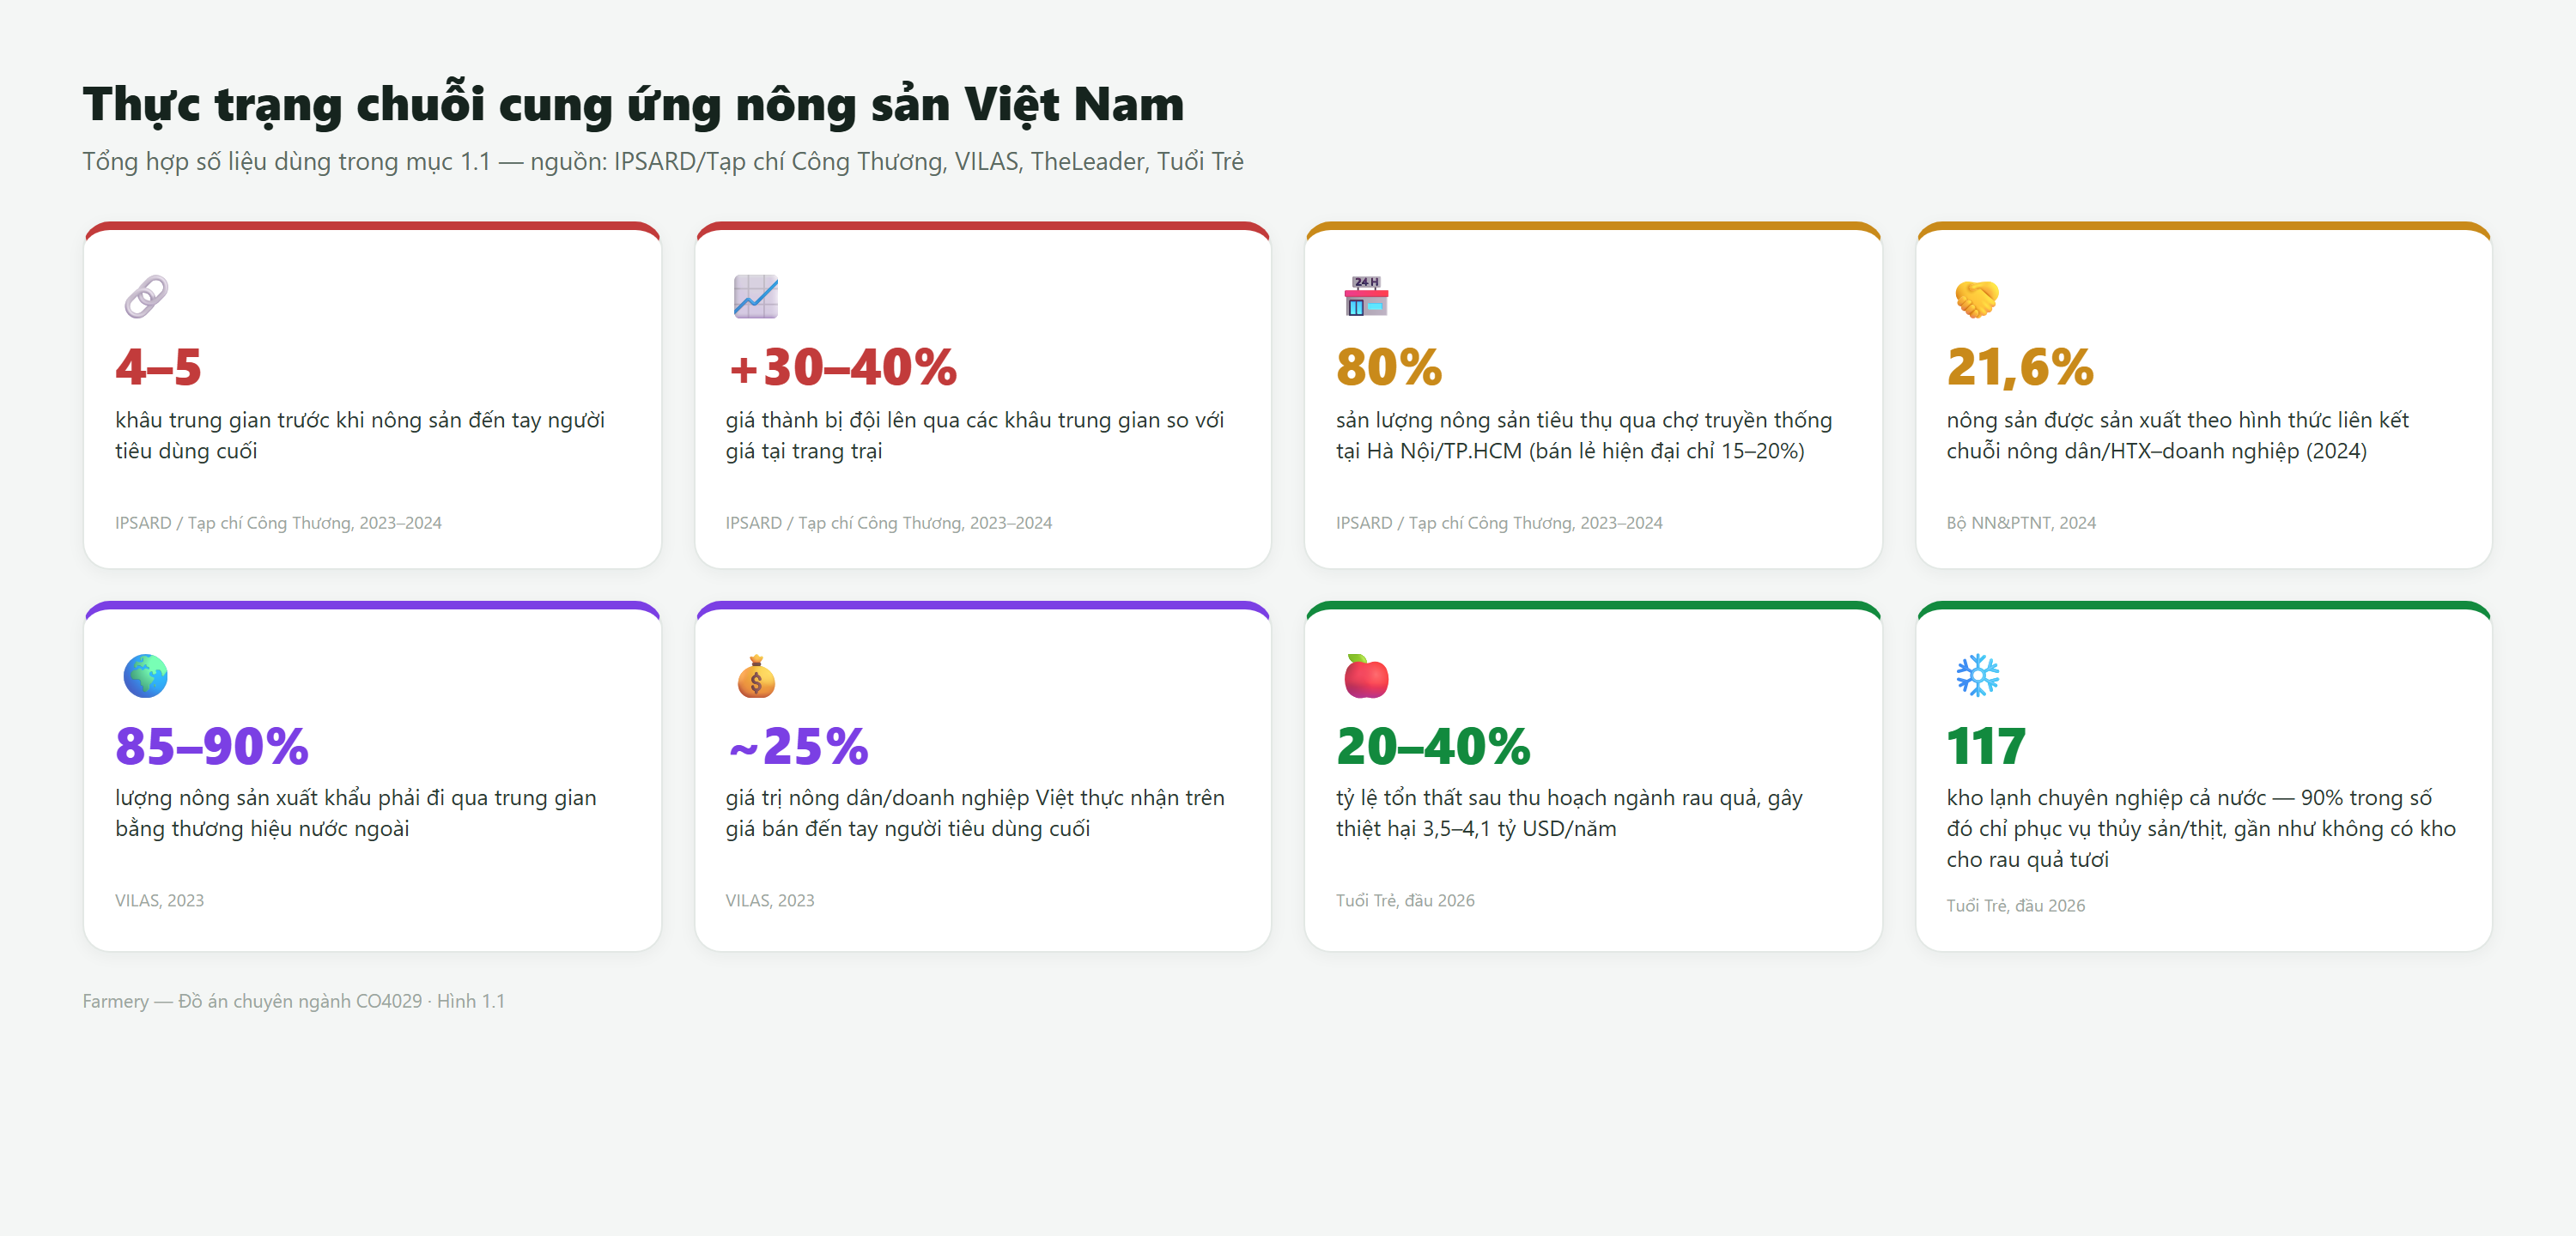
\includegraphics[width=\textwidth]{image/comparison/thuc-trang-chuoi-cung-ung.png}
\caption{Thực trạng chuỗi cung ứng nông sản Việt Nam}
\label{fig:thuctrang}
\end{figure}

Vai trò của thương lái trong bối cảnh này mang tính hai mặt: một mặt họ giải quyết bài toán thu gom, sơ chế và vận chuyển phân tán mà từng nông hộ nhỏ khó tự thực hiện; mặt khác, do nắm thông tin thị trường tốt hơn nông dân (bất cân xứng thông tin --- xem mục~\ref{subsec:reputation}) và thường là điểm bán duy nhất tại địa phương vào thời điểm thu hoạch, thương lái có vị thế đàm phán giá vượt trội, dẫn đến hiện tượng ép giá khi vào vụ thu hoạch rộ \cite{vilas_logistics}.

Nguyên nhân sâu xa của hiện tượng ``được mùa mất giá'' gồm ba nhóm yếu tố chính:
\begin{itemize}
    \item Cung tăng ồ ạt và đồng loạt khi vào vụ thu hoạch do sản xuất còn theo tập quán mùa vụ, thiếu quy hoạch rải vụ.
    \item Thiếu phương án tiêu thụ đa kênh và năng lực chế biến sâu/bảo quản để hấp thụ sản lượng dư thừa.
    \item Tỷ lệ hao hụt, hư hỏng sau thu hoạch rất cao --- theo ông Nguyễn Thanh Bình, Chủ tịch Hiệp hội Rau quả Việt Nam (Vinafruit), được TheLeader (2024) dẫn lại, tỷ lệ này với một số loại trái cây có thể lên tới 35--40\%, buộc nông dân phải bán tháo với giá thấp trước khi hàng hỏng hoàn toàn \cite{theleader_2024}.
\end{itemize}

Đây chính là ba ``điểm đau'' mà một sàn TMĐT như Farmery có thể can thiệp trực tiếp:
\begin{itemize}
    \item Kết nối cung--cầu theo thời gian thực và mở rộng thị trường tiêu thụ ra ngoài phạm vi địa lý của thương lái địa phương.
    \item Cho phép đặt hàng B2B theo lịch/hợp đồng để nông dân chủ động sản xuất.
    \item Tối ưu logistics lạnh và rút ngắn thời gian từ thu hoạch đến giao hàng.
\end{itemize}

Số liệu cập nhật đầu năm 2026 (báo Tuổi Trẻ, xem Hình~\ref{fig:thuctrang}) cho thấy vấn đề tổn thất sau thu hoạch và thiếu kho lạnh chuyên dụng cho rau quả tươi vẫn chưa được cải thiện đáng kể so với năm 2024, buộc nông dân ``bán ngay, bán vội'' ngay khi thu hoạch và càng suy yếu vị thế đàm phán giá trước thương lái \cite{tuoitre_2026}. Điều này cho thấy đầu tư vào logistics lạnh là điều kiện gần như bắt buộc để một sàn TMĐT như Farmery giải quyết triệt để hiện tượng ``được mùa mất giá'', chứ không chỉ dừng ở việc kết nối cung--cầu.

\section{Mục tiêu đồ án}

% TODO (nhóm rà soát lại cho khớp phạm vi thật đã/sẽ hiện thực ở Ch.4):
Đồ án hướng tới xây dựng Farmery --- một nền tảng thương mại điện tử nông sản theo mô hình marketplace nhiều người bán (multi-vendor), phục vụ đồng thời kênh bán lẻ (B2C) và bán sỉ theo hợp đồng (B2B) --- với các công việc cụ thể sau:
\begin{enumerate}
    \item Xây dựng quy trình đăng ký, xác thực và kiểm duyệt chứng nhận (VietGAP/GlobalGAP) cho nhà bán, làm cơ sở minh bạch hóa thông tin nguồn gốc sản phẩm.
    \item Hiện thực cơ chế truy xuất nguồn gốc bằng mã QR gắn với nhật ký canh tác theo từng lô sản phẩm.
    \item Hiện thực song song hai luồng giao dịch từ phía nhà bán: bán lẻ (B2C) cho người tiêu dùng cá nhân và bán sỉ theo báo giá/hợp đồng (B2B) cho doanh nghiệp thu mua, có hỗ trợ giá bậc theo số lượng tối thiểu (MOQ).
    \item Thiết kế quy trình vận chuyển và xử lý khiếu nại phù hợp đặc thù hàng nông sản dễ hư hỏng.
    \item Tích hợp các tính năng AI hỗ trợ ra quyết định: gợi ý sản phẩm, dự báo nhu cầu/giá nông sản, phát hiện gian lận/bất thường, và trợ lý ảo tư vấn cho người dùng.
    \item Xây dựng công cụ quản trị (kiểm duyệt, giám sát vi phạm, báo cáo thống kê) hỗ trợ vận hành sàn.
\end{enumerate}

\section{Ý nghĩa khoa học và ý nghĩa thực tiễn}

\subsection*{Ý nghĩa khoa học}
% TODO: nhóm bổ sung/điều chỉnh cho sát với đóng góp thực tế của đồ án.
Đồ án góp phần hệ thống hóa và vận dụng có chọn lọc các lý thuyết liên quan đến thương mại điện tử đa vai trò (mô hình B2B2C, marketplace nhiều người bán), chuỗi cung ứng thực phẩm ngắn (SFSC) và disintermediation, truy xuất nguồn gốc theo chuẩn GS1, cùng lý thuyết bất cân xứng thông tin (information asymmetry) trong thiết kế hệ thống đánh giá/uy tín, vào một bài toán ứng dụng cụ thể là nông sản Việt Nam. Việc đối chiếu với các nền tảng quốc tế đã công bố kết quả nghiên cứu (như Farm2Market) và các nền tảng thương mại đã triển khai thực tế (Ninjacart, e-Choupal, Pinduoduo) giúp làm rõ khoảng trống nghiên cứu (research gap) mà đồ án hướng tới lấp đầy: tích hợp đồng thời hai luồng bán lẻ/bán sỉ, truy xuất nguồn gốc gắn nhật ký canh tác, và các mô-đun AI hỗ trợ ra quyết định trên cùng một nền tảng (xem mục~\ref{subsec:researchgap}).

\subsection*{Ý nghĩa thực tiễn}
% TODO: nhóm bổ sung/điều chỉnh cho sát với đóng góp thực tế của đồ án.
Về mặt thực tiễn, hệ thống hướng tới hỗ trợ trực tiếp bốn nhóm người dùng đã được phân tích tại mục~\ref{sec:doituongnguoidung}: giúp nông dân/HTX tiếp cận thị trường rộng hơn và giảm phụ thuộc vào thương lái; giúp người tiêu dùng cá nhân mua được nông sản có nguồn gốc rõ ràng; giúp doanh nghiệp thu mua có kênh đặt hàng sỉ theo hợp đồng với nguồn cung minh bạch; và cung cấp công cụ quản trị hiệu quả cho đội ngũ vận hành sàn. Đồng thời, kết quả đồ án có thể là cơ sở để mở rộng thành sản phẩm hoàn chỉnh hơn ở học kỳ Khóa luận tốt nghiệp tiếp theo.

\section{Phạm vi và giới hạn đề tài}
\label{sec:phamvi}

% TODO: nhóm rà soát lại phạm vi cho khớp với những gì thực sự hiện thực ở Ch.4, tránh cam kết vượt quá phạm vi đã làm.
Đồ án tập trung vào bốn nhóm người dùng: nông dân/hợp tác xã, người tiêu dùng cá nhân, doanh nghiệp thu mua (nhà hàng, siêu thị, nhà phân phối) và quản trị viên hệ thống (chi tiết phân tích tại mục~\ref{sec:doituongnguoidung}). Phạm vi nghiệp vụ bao gồm bảy quy trình chính: đăng ký/xác thực nhà bán, đăng và kiểm duyệt sản phẩm, bán lẻ, đánh giá sản phẩm/nhà bán, bán sỉ, quản lý tồn kho/vận chuyển/khiếu nại, và quản trị hệ thống (chi tiết tại mục~\ref{sec:quytrinhnghiepvu}), cùng luồng tiếp cận/tham gia hệ thống cho từng nhóm người dùng (mục~\ref{sec:luongtiepcan}) và mô hình kinh doanh của nền tảng (mục~\ref{sec:businessmodelcanvas}).

Đồ án giới hạn ở việc xây dựng phiên bản khả thi tối thiểu (MVP) của nền tảng, không bao gồm: tích hợp trực tiếp với hệ thống xác minh chứng nhận VietGAP/GlobalGAP của cơ quan cấp chứng nhận (giai đoạn đầu xác minh thủ công); ứng dụng blockchain cho truy xuất nguồn gốc (lý do được phân tích tại mục~\ref{subsec:gs1blockchain}); vận hành kho bãi vật lý trung chuyển --- Farmery chỉ điều phối và tích hợp API với các đơn vị vận chuyển thứ ba (3PL), nhà bán tự quản lý kho của mình (mục~\ref{subsec:khobai}); và các nghiệp vụ xuất khẩu xuyên biên giới.

\section{Cấu trúc báo cáo}

Phần còn lại của báo cáo được tổ chức như sau. Chương~\ref{chap:coso} trình bày tổng quan các nghiên cứu, nền tảng thương mại điện tử nông sản liên quan và cơ sở lý thuyết được vận dụng trong đồ án. Chương~\ref{chap:phantich} phân tích yêu cầu và trình bày thiết kế hệ thống, bao gồm quy trình nghiệp vụ, kiến trúc, cơ sở dữ liệu và các sơ đồ thiết kế chi tiết. Chương~\ref{chap:hienthuc} mô tả quá trình hiện thực các mô-đun chính của hệ thống. Chương~\ref{chap:danhgia} trình bày kịch bản kiểm thử và kết quả đánh giá hệ thống. Chương~\ref{chap:ketluan} tổng kết các kết quả đạt được, hạn chế còn tồn tại và hướng phát triển tiếp theo.
